Kernel code can be written directly using the CUDA instruction set called PTX, but it is usually more beneficial to use a higher level language such as C.
Both of them must be compiled into machine code before it can be used.
This can be done by the Nvidia CUDA Compiler (NVCC).
As \cuda{} code runs on both host and device, NVCC separates the two, and sends the CPU code to a C compiler (GCC for instance) and the device code is further compiled to PTX instructions by NVCC \cite{cuda:programmingguide}.
At the end, the PTX and CPU (assembly) instructions are compiled to machine code which can be transferred to the host and device to be executed.
The flow is depicted in \autoref{fig:nvcc-compiler}
\begin{figure}[ht]
	\centering
	\fbox{
		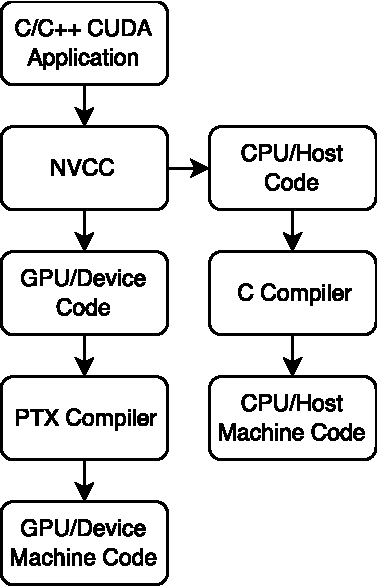
\includegraphics[width=0.3\textwidth]{figs/programming-model/NVCC.pdf}
	}
	\caption{NVCC compiling}
	\label{fig:nvcc-compiler}
\end{figure}
To separate C/C++ code files from \cuda{} code files, \cuda{} uses the file extension ".cu".
A simple example of compiling and running a .cu file in Linux can be seen in \autoref{lst:compile-example}.
\begin{lstlisting}[language=bash,caption={Compilation and run example},label=lst:compile-example]
	nvcc -c helloworld.cu -o helloworld
	./helloworld 
\end{lstlisting}
This is only valid for very simple cuda programs, as there are a lot of different compiler flags to be used, depending on the platform etc.